\documentclass[letterpaper, 11 pt]{article}
\usepackage{amssymb, latexsym, amsmath, amsthm, graphicx, amsthm,alltt,color, listings,multicol,xr-hyper,hyperref,aliascnt,enumitem}
\usepackage{xfrac}

\usepackage{parskip}
\usepackage[,margin=0.7in]{geometry}
\setlength{\textheight}{8.5in}

\usepackage{epstopdf}

\DeclareGraphicsExtensions{.eps}
\usepackage{tikz}


\usepackage{tkz-euclide}
%\usetkzobj{all}
\tikzstyle geometryDiagrams=[rounded corners=.5pt,ultra thick,color=black]
\colorlet{penColor}{black} % Color of a curve in a plot


\usepackage{subcaption}
\usepackage{float}
\usepackage{fancyhdr}
\usepackage{pdfpages}
\newcounter{includepdfpage}
\usepackage{makecell}


\usepackage{currfile}
\usepackage{xstring}




\graphicspath{  
{./otherDocuments/}
}

\author{Claire Merriman}
\newcommand{\classday}[1]{\def\classday{#1}}

%%%%%%%%%%%%%%%%%%%%%
% Counters and autoref for unnumbered environments
% Not needed??
%%%%%%%%%%%%%%%%%%%%%
\theoremstyle{plain}


\newtheorem*{namedthm}{Theorem}
\newcounter{thm}%makes pointer correct
\providecommand{\thmname}{Theorem}

\makeatletter
\NewDocumentEnvironment{thm*}{o}
 {%
  \IfValueTF{#1}
    {\namedthm[#1]\refstepcounter{thm}\def\@currentlabel{(#1)}}%
    {\namedthm}%
 }
 {%
  \endnamedthm
 }
\makeatother


\newtheorem*{namedprop}{Proposition}
\newcounter{prop}%makes pointer correct
\providecommand{\propname}{Proposition}

\makeatletter
\NewDocumentEnvironment{prop*}{o}
 {%
  \IfValueTF{#1}
    {\namedprop[#1]\refstepcounter{prop}\def\@currentlabel{(#1)}}%
    {\namedprop}%
 }
 {%
  \endnamedprop
 }
\makeatother

\newtheorem*{namedlem}{Lemma}
\newcounter{lem}%makes pointer correct
\providecommand{\lemname}{Lemma}

\makeatletter
\NewDocumentEnvironment{lem*}{o}
 {%
  \IfValueTF{#1}
    {\namedlem[#1]\refstepcounter{lem}\def\@currentlabel{(#1)}}%
    {\namedlem}%
 }
 {%
  \endnamedlem
 }
\makeatother

\newtheorem*{namedcor}{Corollary}
\newcounter{cor}%makes pointer correct
\providecommand{\corname}{Corollary}

\makeatletter
\NewDocumentEnvironment{cor*}{o}
 {%
  \IfValueTF{#1}
    {\namedcor[#1]\refstepcounter{cor}\def\@currentlabel{(#1)}}%
    {\namedcor}%
 }
 {%
  \endnamedcor
 }
\makeatother

\theoremstyle{definition}
\newtheorem*{annotation}{Annotation}
\newtheorem*{rubric}{Rubric}

\newtheorem*{innerrem}{Remark}
\newcounter{rem}%makes pointer correct
\providecommand{\remname}{Remark}

\makeatletter
\NewDocumentEnvironment{rem}{o}
 {%
  \IfValueTF{#1}
    {\innerrem[#1]\refstepcounter{rem}\def\@currentlabel{(#1)}}%
    {\innerrem}%
 }
 {%
  \endinnerrem
 }
\makeatother

\newtheorem*{innerdefn}{Definition}%%placeholder
\newcounter{defn}%makes pointer correct
\providecommand{\defnname}{Definition}

\makeatletter
\NewDocumentEnvironment{defn}{o}
 {%
  \IfValueTF{#1}
    {\innerdefn[#1]\refstepcounter{defn}\def\@currentlabel{(#1)}}%
    {\innerdefn}%
 }
 {%
  \endinnerdefn
 }
\makeatother

\newtheorem*{scratch}{Scratch Work}


\newtheorem*{namedconj}{Conjecture}
\newcounter{conj}%makes pointer correct
\providecommand{\conjname}{Conjecture}
\makeatletter
\NewDocumentEnvironment{conj}{o}
 {%
  \IfValueTF{#1}
    {\innerconj[#1]\refstepcounter{conj}\def\@currentlabel{(#1)}}%
    {\innerconj}%
 }
 {%
  \endinnerconj
 }
\makeatother

\newtheorem*{poll}{Poll question}
\newtheorem{tps}{Think-Pair-Share}[section]


\newenvironment{obj}{
	\textbf{Learning Objectives.} By the end of class, students will be able to:
		\begin{itemize}}
		{\!.\end{itemize}
		}

\newenvironment{pre}{
	\begin{description}
	}{
	\end{description}
}


\newcounter{ex}%makes pointer correct
\providecommand{\exname}{Homework Problem}
\newenvironment{ex}[1][2in]%
{%Env start code
\problemEnvironmentStart{#1}{Homework Problem}
\refstepcounter{ex}
}
{%Env end code
\problemEnvironmentEnd
}

\newcommand{\inlineAnswer}[2][2 cm]{
    \ifhandout{\pdfOnly{\rule{#1}{0.4pt}}}
    \else{\answer{#2}}
    \fi
}


\ifhandout
\newenvironment{shortAnswer}[1][
    \vfill]
        {% Begin then result
        #1
            \begin{freeResponse}
            }
    {% Environment Ending Code
    \end{freeResponse}
    }
\else
\newenvironment{shortAnswer}[1][]
        {\begin{freeResponse}
            }
    {% Environment Ending Code
    \end{freeResponse}
    }
\fi

\let\question\relax
\let\endquestion\relax

\newtheoremstyle{ExerciseStyle}{\topsep}{\topsep}%%% space between body and thm
		{}                      %%% Thm body font
		{}                              %%% Indent amount (empty = no indent)
		{\bfseries}            %%% Thm head font
		{}                              %%% Punctuation after thm head
		{3em}                           %%% Space after thm head
		{{#1}~\thmnumber{#2}\thmnote{ \bfseries(#3)}}%%% Thm head spec
\theoremstyle{ExerciseStyle}
\newtheorem{br}{In-class Problem}

\newenvironment{sketch}
 {\begin{proof}[Sketch of Proof]}
 {\end{proof}}


\newcommand{\gt}{>}
\newcommand{\lt}{<}
\newcommand{\N}{\mathbb N}
\newcommand{\Q}{\mathbb Q}
\newcommand{\Z}{\mathbb Z}
\newcommand{\C}{\mathbb C}
\newcommand{\R}{\mathbb R}
\renewcommand{\H}{\mathbb{H}}
\newcommand{\lcm}{\operatorname{lcm}}
\newcommand{\nequiv}{\not\equiv}
\newcommand{\ord}{\operatorname{ord}}
\newcommand{\ds}{\displaystyle}
\newcommand{\floor}[1]{\left\lfloor #1\right\rfloor}
\newcommand{\legendre}[2]{\left(\frac{#1}{#2}\right)}



%%%%%%%%%%%%





\title{Week 2--MATH 4573 Elementary Number Theory}
\begin{document}

\maketitle
\tableofcontents
%%%%%%%%%%%%%%%%%%%%%%%%%
%%%%%%%%%%%%%%%%%%%%%%%%%
\section{Wednesday, January 20: Least common multiple and the start of Linear Diophantine equations}
%%%%%%%%%%%%%%%%%%%%%%%%%%

Reading assignment: Section 1.3 

{\bf Turn in:} How does this section relate to your previous understanding of the least common multiple?

%%%%%%%%%%%%%%%%%%%%%%%%%
\subsection{Announcements (5 minutes)}
%%%%%%%%%%%%%%%%%%%%%%%%%%
Office hours will be Wednesdays a 2pm Eastern and Thursdays at 1 pm Eastern. I am also available by appointment for those of you who cannot attend office hours. Office hours will use the same link as class. It may take a some time to get the corrects times into the Zoom menu on Carmen, as Zoom still does not allow bulk edit.

To address some of the concerns about learning from reading (as opposed to lecture), I will post videos working through the examples in the reading. This will take a bit of time to post.  However, this course is set up for you to learn by doing. The breakout room problems are meant to help you break down and understand the material from both the reading and the lectures. The reading assignments help keep you on schedule and come to class prepared to start asking questions and working on the material. This is also why late assignments are not accepted except in the case of an excuse absence.


Since we have not covered the proof of the Euclidean algorithm in class yet, the problem modifying the Euclidean algorithm we moved from Homework 1 to Homework 2. This is also the first breakout room assignment of today.

%%%%%%%%%%%%%%%%%%%%%%%%%
\subsection{The Euclidean algorithm (40 minutes)}
%%%%%%%%%%%%%%%%%%%%%%%%%%

\begin{thm}[Euclidean algorithm] 
Let $a,b\in\Z$ with $a\geq b>0$. By the division algorithm, there exist $q_1,r_1\in\Z$ such that 
\[a=b q_1+r_1,\quad 0\leq r_1<b.\]
If $r_1>0$, (by the division algorithm) there exist $q_2,r_2\in\Z$ such that 
\[b=r_1 q_2+r_2,\quad 0\leq r_2<r_1.\]
If $r_2>0$, (by the division algorithm) there exist $q_3,r_3\in\Z$ such that 
\[r_1=r_2 q_3+r_3,\quad 0\leq r_3<r_2.\]

Continuing this process, $r_n=0$ for some $n$. If $n>1$, then $(a,b)=r_{n-1}$. If $n=1$, then $(a,b)=b$.
\end{thm}
\begin{proof}
 Note that $r_1>r_2>r_3>\dots\geq0$ by construction. If the sequence did not stop, then we would have an infinite, decreasing sequence of positive integers, which is not possible. Thus, $r_n=0$ for some $n$. 
 
 When $n=1$, $a=bq+0$ and $\gcd(a,b)=b$.
 
 If $n>1$, then by repeated application of the previous lemma, we have 
 \[\gcd(a,b)=\gcd(b,r_1)=\gcd(r_1,r_2)=\cdots=\gcd(r_{n-2},r_{n-1})\]
 Then $r_{n-2}=r_{n-1} q_n+0$. Thus $\gcd(r_{n-2},r_{n-1})=r_{n-1}$.
\end{proof}

 The Euclidean algorithm allows us to write the gcd $(a,b)$ as a linear combination of $a$ and $b$. That is $(a,b)=ma+by$ for some $m,n\in\Z$.

\begin{br}[Exercise 1.22 and part of 1.23, 20 minutes] From last time, we have that  if $a$ and $b$ are integers with $b\neq 0$, then there is a unique pair of integers $q$ and $r$ such that $a=qb+r$ and $\frac{-|b|}{2}<r\leq \frac{|b|}{2}$. 
	\begin{enumerate}
 				\item Use this result instead of Corollary 1.2 to devise an alternative algorithm to Euclid's for calculating greatest common divisors (the least remainders algorithm). That is, define an algorithm from repeatedly applying the formula from last class.
				\item  Show that for this new algorithm, $r_n=0$ for some $n$, and that if $n>1,$ then $\gcd(a,b)=|r_{n-1}|$. \\\emph{Hint:} The interval $\left(\frac{-|b|}{2},\frac{|b|}{2}\right]$ is length $|b|$, the interval $\left(\frac{-|r_1|}{2},\frac{|r_1|}{2}\right]$ is length $|r_1|$, etc. Why does the length of the intervals decrease? 
		\item Use the least remainders algorithm to find $\gcd(1066,1492)$, and compare to the Euclidean algorithm.
	\end{enumerate}
\end{br}
\begin{solution}
 Homework 2, problem 1. The Euclidean algorithm for $\gcd(1066,1492)$ is example 1.3.
\end{solution}

Here is another example:

\begin{example}
 $a=35, b=9$.
\begin{align*}
 35=9(3)+5,& \quad r_1=5 &35=9(4)-1, & \quad r_1=-1\\
 9=5(1)+4,& \quad r_2=4 & 9=-1(-9)+0, & \quad r_2=0 \quad (\textrm{or $9=1(9)+0$})\\
 5=4(1)+1 & \quad r_3=1\\
 4=1(4)+0 & \quad r_4=0.
\end{align*}
\end{example}

\begin{thm}[Theorem 1.8]
Let $a$ and $b$ be integers (not both 0) with greatest common divisor $d$. Then an integer $c$ has the form $ax+by$ for some $x,y\in\Z$ if and only if $c$ is a multiple of $d$. In particular,  $d$ is the least positive integer of the form $ax+by$ for $x,y\in\Z$.
\end{thm}

The proof of this theorem is one of the ``modifying proofs" problems on the homework, so we will skip it.

\begin{defn}
Two integers $a$ and $b$ are \emph{coprime} or \emph{relatively prime} if $\gcd(a,b)=1$. 
\end{defn}

\begin{cor}[Corollary 1.9]
 Two integers are coprime if and only if there exists integers $x$ and $y$ such that \[ax+by=1.\]
\end{cor}
\begin{proof}
 Let $\gcd(a,d)=d$. If we put $c=1$ in Theorem 1.8, we see that $ax+by=1$ for some $x,y\in\Z$ if and only if $d\mid 1$. Thus, $d=1$ (why?).
\end{proof}

%%%%%%%%%%%%%%%%%%%%%%%%%%
\subsection{Review of reading and least common multiple (5 minutes)} 
%%%%%%%%%%%%%%%%%%%%%%%%%%
Start with questions from the reading.

This section formalizes the concept of the least common multiple. There is only one result. 

\begin{defn} If $a$ and $b$ are integers, then a \emph{common multiple of $a$ and $b$} is an integer $c$ such that $a\mid c$ and $b\mid c$.

 If both $a$ and $b$ are not $0$, the least (positive) number among their common multiples  is called the \emph{least common multiple of $a$ and $b$} and is denoted $lcm(a,b)$ or  $[a,b]$. 
 
If we want the least common multiple of several integers at once we denote that by $[b_1,b_2,b_3,\dots,b_n]$.
\end{defn}

We have a theorem from the reading: 
\begin{thm}[Theorem 1.12]
 Let $a$ and $b$ be positive integers, with $d=\gcd(a,b)$ and $\ell=\operatorname{lcm}(a,b)$. Then \[d\ell=ab.\]
\end{thm}

This is a case where we will focus more on the result than the proof method. I will skip the proof here.

%%%%%%%%%%%%%%%%%%%%%%%%%%
\subsection{Introduction to Diophantine equations (5 minutes)}
%%%%%%%%%%%%%%%%%%%%%%%%%%

Here we will get ahead of the reading!

\begin{defn}
 A \emph{Diophantine equation} is an equation in one or more variables where we want integer solutions. 
 \end{defn}

 Some of the most famous Diophantine equations are integer solutions to the Pythagorean theorem \\$x^2+y^2=z^2$, Fermat's equation $x^n+y^n=z^n$ (we will cover both of these equations in Chapter 11), and Pell's equation $x^2-ny^2=1$.

We will start with the more basic linear Diophantine equation $ax+by=c$. 

{\bf Thought for next time:} Why don't we start with $ax=c$?



%%%%%%%%%%%%%%%%%%%%%%%%%
\section{Friday, January 22: Diophantine equations}
%%%%%%%%%%%%%%%%%%%%%%%%%%
Section 1.4

{\bf Turn in} Does the equation $15m+48n=-6$ have solutions? Why or why not? If it has solutions, how many solutions exist?

%%%%%%%%%%%%%%%%%%%%%%%%%
\subsection{Linear Diophantine equations (40 minutes)}
%%%%%%%%%%%%%%%%%%%%%%%%%%
\begin{thm}[Theorem 1.13]
 Let $a$ and $b$ be integers, with $a$ and $b$ not both $0$, and let $d=\gcd(a,b)$. Then the equation \[ax+by=c\] has an integer solution if and only if $c$ is a multiple of $d$, in which case there are infinitely many solutions. These are the pairs \[x=x_0+\frac{bn}{d},\quad y=y_0-\frac{an}{d}\quad n\in\Z,\] where $x_0,y_0$ is a particular solution.
\end{thm}

The proof of Theorem 1.13 is one of the modifying proofs problems on the homework. 

\begin{example}
 Let $a=6, b=8, c=4$. Then the integer solutions to $6x+8y=4$ are the exact same as the integer solutions to $3x+4y=2$. Let $(x_0,y_0)$ be a solution (we will find one in a second). Then Theorem 1.13 says that the solutions to $6x+8y=4$ are 
 
\begin{align*}
& x=x_0+\frac{8n}{2}=x_0+4n, &y=y_0-\frac{6n}{2}=y_0-3n
\end{align*}

The reduced fraction form matches with the solutions to $3x+4y=2$ from the theorem! It's always good when things that should match do match!

This is a good place for guess and check. $x_0=2, y_0=-1$. Thus, $x=2+4n, y=-1-3n$ for all $n\in\Z$.
\end{example}

\begin{br}[Exercise 1.15, 5 minutes]
Find the general solution of the Diophantine equation \[1485x+1745y=15.\] 
\end{br}

We will go over this one in class

Discussion of lattice points, starting at at 25:24 in the Zoom recording. You can graph the equation as a line, then see where $x,y\in\Z$,  which is where the gridlines meet if the gridlines are at every integer.

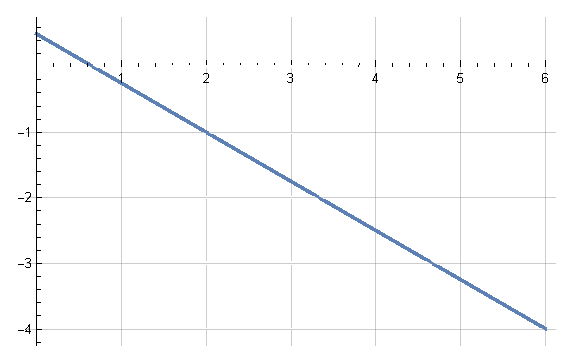
\includegraphics[width=\textwidth]{diophantinelattice}

\begin{br}[Exercise 1.16, 10 minutes]
 If $a_1,\dots,a_k$ and $c$ are integers, when does the Diophantine equation \[a_1x_1+\cdots+a_kx_k=c\] have integer solutions $x_1,\dots,x_k$?
 
 Provide a proof for your answer.
 
\begin{enumerate}
 \item You already know the answer for $k=1$ and $k=2$. What is it?
 \item Try $k=3$.
 \item Try $k=4$.
\item Can you generalize?
\end{enumerate}
\end{br}

%%%%%%%%%%%%%%%%%%%%%%%%%
\subsection{Primes (10 minutes)}
%%%%%%%%%%%%%%%%%%%%%%%%%%
\begin{defn}
An integer $p>1$ is \emph{prime} if the only positive divisors of $p$ are $1$ and itself. An integer $n$ which is not prime is \emph{composite}. 
\end{defn}

Why is $1$ not prime?

It has to do with units and invertibility. The number $1$ holds a special place. It is the multiplicative identity, i.e., anything multiplied by $1$ is just that thing again. Something is said to be invertible in a ``group" (more on that later) if there exist something, which, when multiplied to it, gives you $1$. How many invertible elements are there among the integers? Just two. $1$ and $-1$. And that's the key. If we want to extend our results from positive integers to non-zero integers, we often just need to take into account $\pm 1$. That sounds obvious, but it turns out to be surprisingly critical and yet non-intuitive when we start moving from real integers to complex ones.

\end{document}
\begin{lem}[Lemma 2.1 and Corollary 2.2]
 If $p$ is prime and $a_1,\dots, a_k$ are integers such that $p$ divides $a_1a_2\cdots a_k$, then 
 
\begin{enumerate}
 \item either $p\mid a_i$ or $\gcd(a_i,p)=1$ for each $a_i$,
 \item $p$ divides $a_i$ for some $i$.
\end{enumerate}
\end{lem}
\begin{proof}
 
\begin{enumerate}
 \item By definition $\gcd(a_i,p)$ is a positive divisor of $p$. Thus, it is either $p$ or $1$ since $p$ is prime.
 \item We use induction on $k$. If $k=1,$ then $p\mid a_i$ and we are done.
 
 If $k=2$, then either $p\mid a_1$ and we are done, or $\gcd(a_1,p)=1$ by part (a). Then by Bezout's identity, there exists integers $u,v$ such that $1=a_1u+pv$. Thus, $a_2=a_1a_2u+a_2pv$. By assumption $p\mid a_1a_2$, so $p$ divides the linear combination $a_1a_2u+a_2pv=a_2$.
 
 Now assume that $k>2$ and that the result holds for all products of $k-1$ factors. Then we can write $a=a_1\dots a_{k-1}$ and $b=a_k$ and $p\mid ab$. By the $k=2$ case, it follows that either $p\mid a$ or $p\mid b$. In the first case, $p\mid a=a_1\cdots a_{k-1}$ means that $p\mid a_i$ for some $i$ by the induction hypothesis. In the other case, $p\mid b$ means that $p\mid a_k$ by construction. \qedhere
 \end{enumerate}
\end{proof}

For a polynomial $f(x)=a_n x^n+a_{n-1}x^{n-1}+\cdots+a_1 x+a_0$, where $a_i\in\Z$, whether or not the $a_i$ are divisible by some prime $p$ helps determine if the polynomial can be factored.


\begin{br}[Exercise 2.1, 5 minutes]
 Prove that if $p$ is prime and $p\mid a^k$, then $p\mid a$, and thus $p^k\mid a^k$. 
 
 Is this still valid if $p$ is composite? Prove or provide a counterexample.
\end{br}

\begin{thm} [The Fundamental Theorem of Arithmetic, restatement of Textbook Theorem 2.3] Every integer $n\ge 2$ can be factored into a product of primes $n=p_1 p_2 p_3\dots p_n$ in a unique way (up to rearrangement).\end{thm}
\begin{proof}
We work by induction. We can check that $2=2$, $3=3$ and $4=2^2$ all have prime factorizations. So assume now that all numbers $n$ in the range $2\le n<N$ can be factored in the specified way, and we will show that $N$ can be factored this way as well. If $N$ is prime, then $N$ is its own prime factorization. Otherwise $N$ is composite and has some factor $2\le n_1< N$. Thus we can write $N=n_1n_2$. But $n_2$ must also be in the range $2\le n_2 < N$. Therefore $n_1$ and $n_2$ must be factorable into primes, say $n_1=p_1p_2\dots p_r$ and $n_2= q_1q_2\dots q_s$. Then $N=p_1p_2\dots p _r q_1q_2\dots q_s$. By induction, all integers $n\ge 2$ can be factored into a product of primes.

Now we must show this product is unique up to rearrangement. Suppose that $n$ has two factorizations $p_1p_2\dots p_r$ and $q_1q_2\dots q_s$, and let us assume that $r\le s$. By our previous theorem, since $p_1$ divides $q_1q_2\dots q_s$, it must divide one of the $q_i$'s, and, by rearranging, we can assume that $p_1\mid q_1$. But $q_1$ is prime and only has $1$ and $q_1$ as prime factors, so therefore, $p_1=q_1$. Therefore we have $p_2p_3\dots p_r = q_2q_3\dots q_s$. 

We can repeat this process (and repeatedly rearrange the $q_i$'s as necessary) to show that $p_2=q_2$, and then $p_3=q_3$, and so on until we show that $1=q_{r+1}q_{r+2}\dots q_s$. If $s>r$, then the number on the right-hand side here is greater than $1$, which is impossible, so we have that $r=s$ and $p_i=q_i$ for $1\le i \le r$. This proves that the factorization is unique up to rearrangement.
\end{proof}

So let's suppose we want to factor an integer $n$. Let's start with $d=2$. 

We check to see if $d\mid n$. If it does, then we factor $d$ out of $n$ to get $n'=n/d$. We record the divisor $d$ and henceforth work with $n'$ in place of $n$, restarting at this step. Otherwise, we increment $d$ by one and repeat this step.

Once $n=1$, we have all the factors.

\end{document}

%%%%%%%%%%%%%%%%
Now there are various ways we could try to speed this up. You might think we could only work with those trial divisors $d$ that are prime, but it would take more time to check if $d$ is a prime than it would to just see if it divides $n$. If it's composite, it won't, because we'll have already taken all its factors out of $n$ beforehand.

One thing we can do is only check $d$ up to $\sqrt{n}$. This is because $n$ cannot have two prime factors that are each $>\sqrt{n}$. So if we reach this point, whatever $n$ remains must be prime. So that takes us down from a worst case scenario of $d=n$ to a worst case scenario of $d=\sqrt{n}$. That's a big improvement. It's still very slow.


\vspace{1cm}

We can  write out a prime factorization (of a positive integer) by
\[
a=\prod_p p^{e_p}
\]
where $e_p$ is the number of times $p$ divides $a$ evenly. Note that $\prod$ denote a product in the same way that $\sum$ denotes a sum, and that the subscript $p$ means that the product ranges over all primes.

This is what we are doing when we write $12=2^2\cdot 3$.

This gives us the textbook's formulation of the Fundamental Theorem of Arithmetic

\begin{br}[5 minutes] How would the fundamental theorem of arithmetic (Theorem 1.16) change if we said 1 is a prime number?
\end{br}
Talk about as a class.




